% !TEX TS-program = xelatex
% !TEX encoding = UTF-8 Unicode 

% \documentclass[AutoFakeBold]{LZUThesis}
\documentclass[AutoFakeBold]{LZUThesis}
\usepackage{multirow}
\usepackage{threeparttable}
\CTEXsetup[name={第,部分}]{chapter}
\lstset{
language = MATLAB,
backgroundcolor=\color{white},   % choose the background color; you must add \usepackage{color} or \usepackage{xcolor}  
basicstyle=\footnotesize,        % the size of the fonts that are used for the code  
breakatwhitespace=false,         % sets if automatic breaks should only happen at whitespace  
breaklines=true,                 % sets automatic line breaking  
captionpos=bl,                    % sets the caption-position to bottom  
% commentstyle=\color{green},    % comment style  
% deletekeywords={...},            % if you want to delete keywords from the given language  
% escapeinside={\%*}{*)},          % if you want to add LaTeX within your code  
extendedchars=true,              % lets you use non-ASCII characters; for 8-bits encodings only, does not work with UTF-8  
frame=shadowbox,                    % adds a frame around the code  
keepspaces=true,                 % keeps spaces in text, useful for keeping indentation of code (possibly needs columns=flexible)  
keywordstyle=\color{blue},       % keyword style  
% language=Python,                 % the language of the code  
morekeywords={*,...},            % if you want to add more keywords to the set  
numbers=left,                    % where to put the line-numbers; possible values are (none, left, right)  
numbersep=5pt,                   % how far the line-numbers are from the code  
numberstyle=\tiny\color{gray}, % the style that is used for the line-numbers  
rulecolor=\color{black},         % if not set, the frame-color may be changed on line-breaks within not-black text (e.g. comments (green here))  
showspaces=false,                % show spaces everywhere adding particular underscores; it overrides 'showstringspaces'  
showstringspaces=false,          % underline spaces within strings only  
showtabs=false,                  % show tabs within strings adding particular underscores  
stepnumber=1,                    % the step between two line-numbers. If it's 1, each line will be numbered  
stringstyle=\color{orange},     % string literal style  
tabsize=2,                       % sets default tabsize to 2 spaces  
% title=signalAnalysis.m           % show the filename of files included with \lstinputlisting; also try caption instead of title  
}  

\begin{document}
%=====%
%
%封皮页填写内容
%
%=====%

% 标题样式 使用 \title{{}}; 使用时必须保证至少两个外侧括号
%  如: 短标题 \title{{第一行}},  
% 	      长标题 \title{{第一行}{第二行}}
%             超长标题\tiitle{{第一行}{...}{第N行}}

\title{{基于泰坦尼克号的乘客信息预测其生存率}}



% 标题样式 使用 \entitle{{}}; 使用时必须保证至少两个外侧括号
%  如: 短标题 \entitle{{First row}},  
% 	      长标题 \entitle{{First row}{ Second row}}
%             超长标题\entitle{{First row}{...}{ Next N row}}
% 注意:  英文标题多行时 需要在开头加个空格 防止摘要标题处英语单词粘连.

\author{\CJKfontspec{楷体}李文涛}
\major{电子信息基地班}
\college{320200928101}
\grade{2020级}



\maketitle
\frontmatter

%中文摘要
\ZhAbstract{
    本文首先以AMI码为对比对象介绍$\mathrm{HDB_3}$的由来,简略介绍该编码方案的优缺点,
    接着利用MATLAB进行编程,完成对原数字信号序列进行$\mathrm{HDB_3}$编码
    以及后续对信号的频谱分析,对编码
    时频域分析进行谱图可视化,并同时分析其在其传输速率和频谱利用率上的特点。
    最后根据其频谱特性分析其应用价值。
}
{优缺点,MATLAB,时频域分析,应用分析}


%英文摘要
\EnAbstract{This paper introduces the advantages and advantages of $\mathrm{HDB_3}$, 
and then uses MATLAB to program,
 complete the $\mathrm{HDB_3}$ encoding of the original digital signal sequence and the subsequent spectrum analysis of the signal, 
 and the spectral diagram visualization of the encoding time frequency domain analysis, 
 and analyze its characteristics in its transmission rate and frequency utilization.
 Finally, its application value is analyzed according to its spectral characteristics.
    \fontspec{Times New Roman}}
{Advantages and disadvantages, time frequency domain analysis, application analysis}

%生成目录
% \tableofcontents
% \addcontentsline{toc}{chapter}{目录}
% \thispagestyle{empty}


%文章主体
\mainmatter

\chapter{理解数据}

\section{导入数据}

\begin{lstlisting}
import pandas as pd
import numpy as np
import matplotlib.pyplot as plt

data_train=pd.read_csv("./train.csv")
data_test = pd.read_csv("./test.csv")

\end{lstlisting}
将项目处理所需的库和数据集导入。

\section{浏览数据集}

\begin{lstlisting}
    data_train.head(5)
    data_test.head(5)
\end{lstlisting}
用.head()取前五个数据,以用来对数据所包含的信息进行理解。
\begin{figure}[htbp]
    \centering
    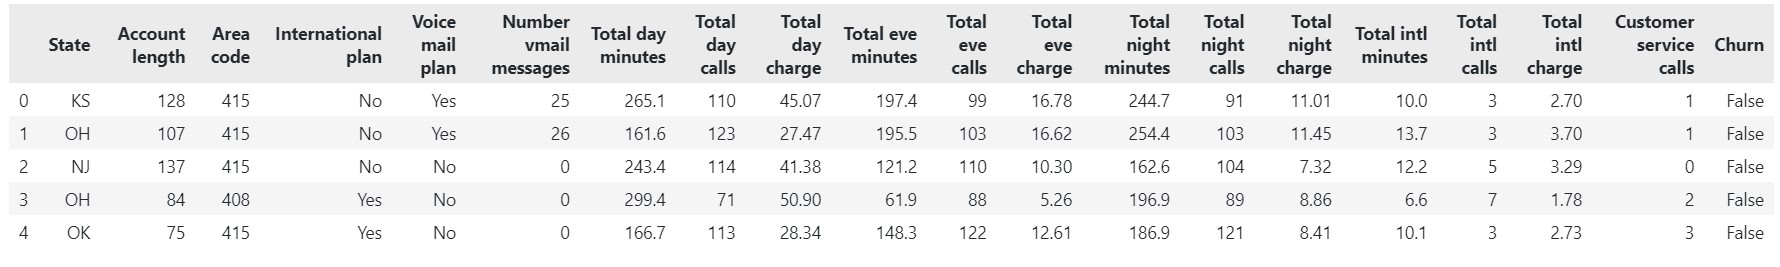
\includegraphics[keepaspectratio,width=500pt]{trainhead.jpg}
    \caption{训练集数据实例}
\end{figure}
\begin{figure}[htbp]
    \centering
    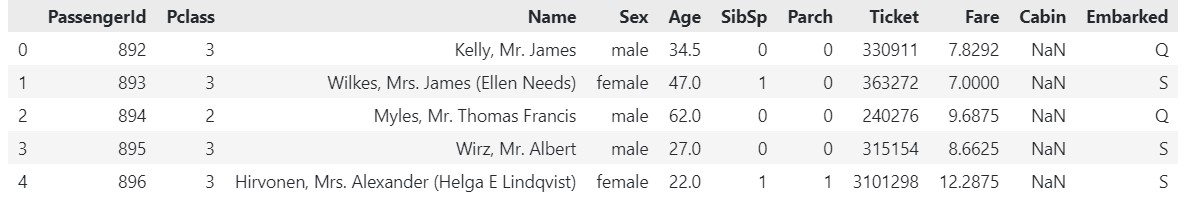
\includegraphics[keepaspectratio,width=500pt]{test.head.jpg}
    \caption{测试集数据实例}
\end{figure}
\section{对数据属性的理解}
通过上一步我们发现该数据集有$\mathrm{PassengerId}$、$\mathrm{Survived}$、$\mathrm{Pclass}$等
一系列属性,通过查阅相关资料,各属性所包含的意思在下方说明。

$\mathrm{PassengerId}$:乘客的编号

$\mathrm{Survived}$:该名乘客是否生还(1为生还,0为遇难)

$\mathrm{Pclass}$:该乘客所乘坐的座舱的等级

$\mathrm{Name}$:该乘客的姓名

$\mathrm{Sex}$:该乘客的性别

$\mathrm{Age}$:该乘客的年龄

$\mathrm{SibSp}$:该乘客在船上有多少堂兄弟妹

$\mathrm{Parch}$:该乘客在船上有多少父母或者孩子

$\mathrm{Ticket}$:该乘客的船票编号

$\mathrm{Fare}$:该乘客的船票票价

$\mathrm{Cabin}$:该乘客的船舱编号

$\mathrm{Embarked}$:该乘客的登船港口
\chapter{数据清洗}
\section{查看训练集详细信息}
\begin{lstlisting}
    print(data_train.describe())  
    print(data_test.describe())  
\end{lstlisting}
    \begin{figure}[htbp]
        \centering
        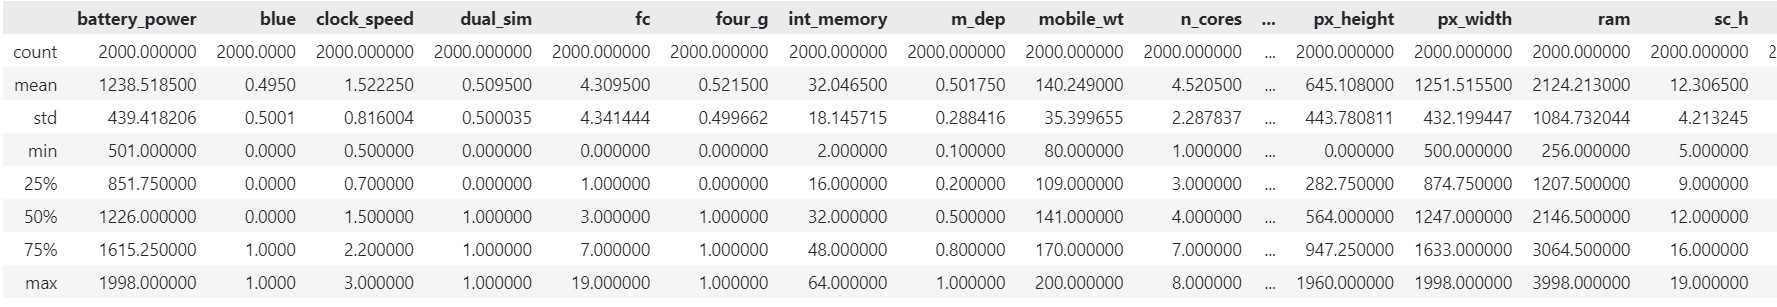
\includegraphics[keepaspectratio,width=400pt]{traindetail.jpg}
        \caption{训练集及测试集各数据属性分析}
    \end{figure}
\section{查看数据缺失情况}
\begin{lstlisting}
    print(data_train.info())  
    print(data_test.info())
\end{lstlisting}
    \begin{figure}[htbp]
        \centering
        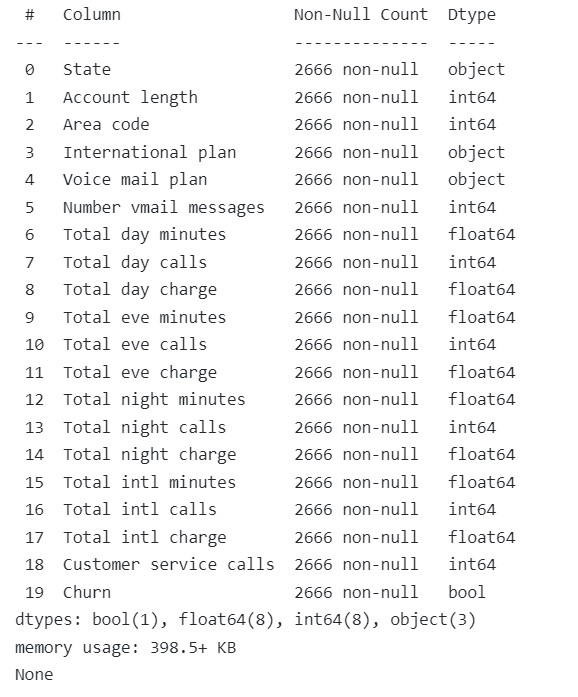
\includegraphics[keepaspectratio,width=380pt]{trainerror.jpg}
        \caption{训练集各数据属性分析}
    \end{figure}
\begin{figure}[htbp]
    \centering
    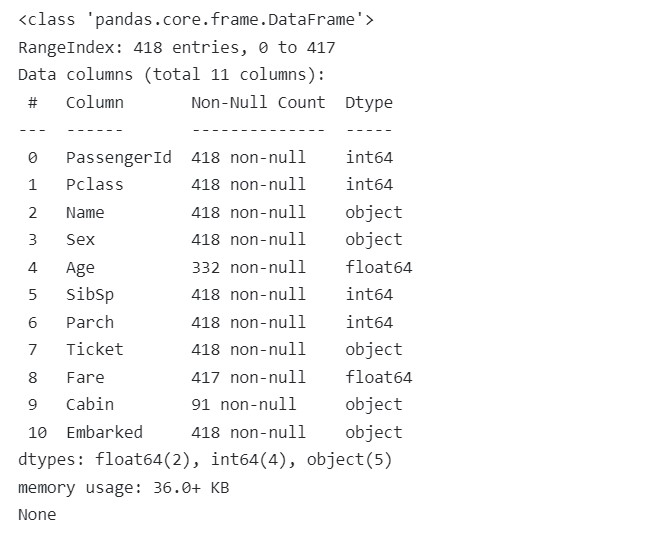
\includegraphics[keepaspectratio,width=380pt]{testerror.jpg}
    \caption{测试集各数据属性分析}
\end{figure}
    经观察上图我们发现,属性$\mathrm{Age}$、$\mathrm{Cabin}$、$\mathrm{Embarked}$、$\mathrm{Fare}$
    在两个数据集中有缺失的部分,下面我们对这些部分进行数据的填充。
    \section{数据填充}
    经查阅资料,我们采用以下的代码对数据集中$\mathrm{Age}$、$\mathrm{Cabin}$、$\mathrm{Embarked}$、$\mathrm{Fare}$
    四个属性有缺失的数据进行填充。
    \begin{lstlisting}
        # 填充数据值
        def fillna_data(df_train, df_test):
            # 对训练集和测试集中的"Age"数据进行平均值填充
            df_train['Age'] = df_train['Age'].fillna(df_train['Age'].mean())
            df_test['Age'] = df_test['Age'].fillna(df_test['Age'].mean())
            # 添加一个新的类别"Missing"来填充"Cabin"
            df_train['Cabin'] = df_train['Cabin'].fillna('Missing')
            df_test['Cabin'] = df_test['Cabin'].fillna('Missing')
            # 用出现频率最多的类别填充训练集中的"Embarked"属性
            df_train['Embarked'] = df_train['Embarked'].fillna(
            df_train['Embarked'].mode()[0])
            # 用出现频率最多的类别填充测试集中的"Fare"属性
            df_test['Fare'] = df_test['Fare'].fillna(
            df_test['Fare'].mode()[0])
            return df_train, df_test
        
        # 得到填充后的数据集 df_train, df_test
        df_train, df_test = fillna_data(data_train, data_test)
    \end{lstlisting}
    \section{数据处理}
    经查阅资料,为便于处理,我们将数据各属性的数据进行one-hot编码、归一化处理等,以备下一步数据的分析。
    \begin{lstlisting}
        # 对数据集中的字符串数据进行编码处理
        def preprocess_data(train, test):
            # 使用one-hot编码将登船港口"Embarked"进行转换
            # 训练集
            Embarked = pd.get_dummies(train['Embarked'], prefix='Embarked')
            tmp_train = pd.concat([train, Embarked], axis=1)
            tmp_train.drop(columns=['Embarked'], inplace=True)
            # 测试集
            Embarked = pd.get_dummies(test['Embarked'], prefix='Embarked')
            tmp_test = pd.concat([test, Embarked], axis=1)
            tmp_test.drop(columns=['Embarked'], inplace=True)
            # 将年龄归一化
            tmp_train['Age'] = (tmp_train['Age'] - tmp_train['Age'].min()) / (tmp_train['Age'].max() - tmp_train['Age'].min())
            tmp_test['Age'] = (tmp_test['Age'] - tmp_test['Age'].min()) / (tmp_test['Age'].max() - tmp_test['Age'].min())
            # 将船票价格归一化
            if 'Fare' in tmp_train.columns:
                tmp_train['Fare'] = (tmp_train['Fare'] - tmp_train['Fare'].min()) / (tmp_train['Fare'].max() - tmp_train['Fare'].min())
            if 'Fare' in tmp_test.columns:
                tmp_test['Fare'] = (tmp_test['Fare'] - tmp_test['Fare'].min()) / (tmp_test['Fare'].max() - tmp_test['Fare'].min())
            # 将性别"Sex"这一特征从字符串映射至数值
            # 0代表female,1代表male
            gender_class = {'female': 0, 'male': 1}
            tmp_train['Sex'] = tmp_train['Sex'].map(gender_class)
            tmp_test['Sex'] = tmp_test['Sex'].map(gender_class)
            
            return tmp_train, tmp_test        
    \end{lstlisting}
\chapter{数据分析}
下面对处理后的数据通过相关直方图和相关系数热力图进行观察比较,选取我们所需要的对乘客是否生还的判断属性。
\section{乘客存活概率与座舱等级的关系}
\begin{lstlisting}
    # 乘客存活概率与客舱的关系
    import seaborn as sns
    sns.barplot(x='Pclass', y='Survived', data=df_train)
    plt.show()
\end{lstlisting}
\begin{figure}[htbp]
    \centering
    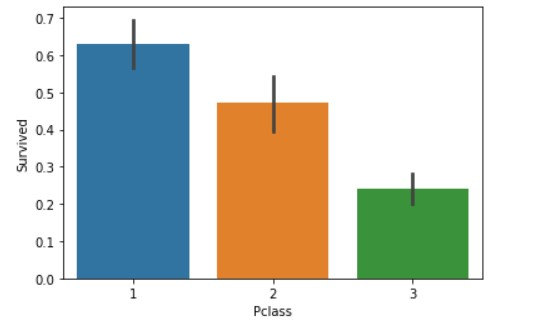
\includegraphics[keepaspectratio,width=310pt]{tPclass.jpg}
    \caption{乘客存活概率与客舱之间的关系}
\end{figure}
\section{乘客存活概率与性别的关系}
\begin{lstlisting}
    sns.barplot(x='Sex', y='Survived', data=df_train)
    plt.show()
\end{lstlisting}
\begin{figure}[htbp]
    \centering
    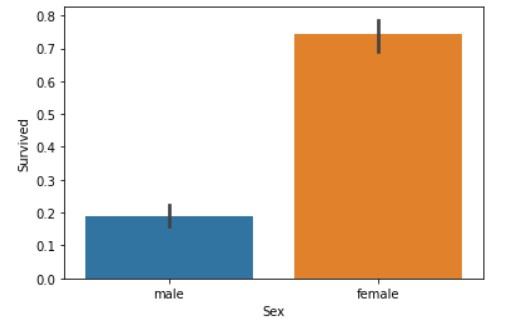
\includegraphics[keepaspectratio,width=310pt]{tSex.jpg}
    \caption{乘客存活概率与性别之间的关系}
\end{figure}
\section{各属性之间的相关关系程度}
\begin{lstlisting}
    df = data_train[['Pclass', 'Sex', 'Age', 'SibSp', 'Parch', 'Fare', 'Survived']]
    # 属性间相关系数
    cor = df.corr()
    print(cor)
    # 属性间相关系数热力图
    sns.heatmap(cor,cmap="Greens")
    plt.show()
\end{lstlisting}
\begin{figure}[htbp]
    \centering
    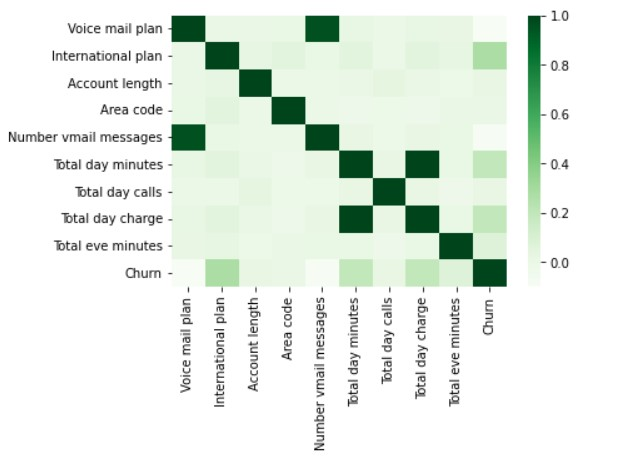
\includegraphics[keepaspectratio,width=320pt]{tconnect.jpg}
    \caption{各属性之间的相关关系程度}
\end{figure}
通过常识和观察热力图我们发现$\mathrm{PassengerId, Name, Ticket, Cabin, SibSp, Parch}$
这几个属性与乘客是否获救的关系不大,我们认为其与乘客是否获救无关,在下一步的分析之前我们将其舍弃。

\chapter{构建模型}
这里采用SVM来进行模型的构建。以下步骤按照参考资料中的代码进行模型的构建。
\section{去除无关数据}
\begin{lstlisting}
    # 去除无关数据
    df_train = df_train.drop(columns=['PassengerId', 'Name', 'Ticket', 'Cabin', 'SibSp', 'Parch'])
    df_test = df_test.drop(columns=['PassengerId', 'Name', 'Ticket', 'Cabin', 'SibSp', 'Parch'])
\end{lstlisting}
利用.drop函数把“无关”的数据属性去除。
\section{处理并划分数据集}
\begin{lstlisting}
    data_train, data_test = preprocess_data(df_train, df_test)
    # 划分出标签类别,记录生存还是死亡,生存1,死亡0
    label_train = data_train.loc[:, 'Survived']
    data_train = data_train.drop(columns=['Survived'])
    from sklearn.model_selection import train_test_split
    train_X, test_X, train_y, test_y = train_test_split(data_train,
                                                    label_train,
                                                    train_size=.8)
\end{lstlisting}
这里取训练集的$80\%$以备之后的模型测试及评估。
\section{模型训练}
\begin{lstlisting}
    from sklearn import svm
    # 实例化对象,参数调整
    clf_SVM = svm.SVC()
    # 训练SVM模型
    clf_SVM.fit(train_X, train_y)    
\end{lstlisting}
\chapter{评估模型}
下面我们分别从混淆矩阵、分类报告和.score函数来对我们所训练出的模型进行评估。
\begin{lstlisting}
    from sklearn.metrics import confusion_matrix, classification_report

    pred_SVM = clf_SVM.predict(test_X)
    score = clf_SVM.score(test_X,test_y)
    # 输出混淆矩阵
    print(confusion_matrix(test_y, pred_SVM))
\end{lstlisting}
\begin{figure}[htbp]
    \centering
    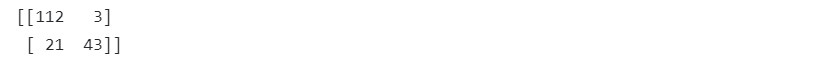
\includegraphics[keepaspectratio,width=500pt]{testaxe.jpg}
    \caption{混淆矩阵}
\end{figure}
\begin{lstlisting}
    # 输出分类报告
    print(classification_report(test_y, pred_SVM))
\end{lstlisting}
\begin{figure}[htbp]
    \centering
    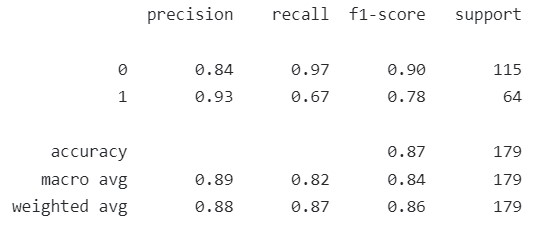
\includegraphics[keepaspectratio,width=350pt]{testlabel.jpg}
    \caption{分类报告}
\end{figure}
\begin{lstlisting}
    # 输出测试集评估结果
    print(score)
\end{lstlisting}
\begin{figure}[htbp]
    \centering
    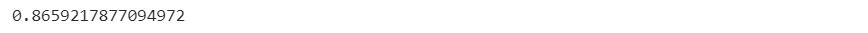
\includegraphics[keepaspectratio,width=500pt]{score.jpg}
    \caption{测试集评估结果}
\end{figure}
\chapter{方案实施及结果提交}
\begin{lstlisting}
    data_predict = clf_SVM.predict(data_test)
    data_predict_result = pd.DataFrame(data_predict,columns=['survived'])
    #将需要预测的数据集放入我们构建的模型中并将结果存入data_predict_result
    data2 = pd.read_csv('test.csv')
    id = data2['PassengerId']
    result = pd.concat([id,data_predict_result],axis=1)
    result.to_csv('predict_result.csv')
    #规范结果,并将结果以csv格式保存
\end{lstlisting}
\chapter{总结与收获}
通过完整地对一个数据集进行分析,直到构筑模型并能够利用模型进行预测,
个人了解了利用人工智能算法对一般问题解决的大致流程,能够通过查阅资料并对数据进行
理解分析来完成信息的预测。

同时也发现了自己对人工智能算法方面的了解不足,在今后的学习过程中会更加主动地
了解学习人工智能智能算法的实现。
\backmatter


% %=======%
% %引入参考文献文件
% %=======%
\bibdatabase{bib/POC}%bib文件名称 仅修改bib/ 后部分
\printbib
\nocite{*} %显示数据库中有的,但是正文没有引用的文献


% \Appendix

% 这里是附录页,可要可不要

% \Thanks.



\end{document}